
\section{Introduction}
\iffalse
{\color{red} 
TODO:
\begin{itemize}
    \item item == document
    \item web-api
    \item doc-comments in source code
    \imte use case
\end{itemize}
}
\fi

%\subsection{Motivation}
% Choice overload
% Aktuelle Situation in der Kleidungsbranche
% kurzer Einblick in Recommender systems (wird spaeter weiter ausgefuehrt)
\noindent
When a typical customer enters a shop or department store, he often gets confronted with a very huge collection of products he can choose from.
This is especially true, when searching for products online on a web shop.
The commonly well-known web shop \gls{amazon.com}, for instance, provides about 280 million different products on their internet presence solely for the United States - there are even more products offered world wide.\citep{marketplaceanalytics:2014}
Even shops dedicated to only a special kind of product can have a wide array of products.
On \gls{zalando}, a German online shop dedicated to clothing, one can choose out of 150.000 products and 1.500 different brands.\citep{visser:2014}
\\

%\paragraph{Choice Overload}
\index{Choice Overload}
There is a general belief that great choice pleases the customer's needs.
However it is actually proven that this idea is not fully correct and reality is much more complex.
Already in 2000 a group of scientists demonstrated that a great variety can also have negative effects.
It is proven that large assortments can lower the customer's willingness to purchase products.\citep[p.~312-313]{diehl:2010}
Furthermore, to much choice can also lower the customer's satisfaction.\citep[p.~320]{diehl:2010}
The state of being confronted with an overwhelming range of choice and therefore having trouble finding the right product is commonly known as choice overload.\citep[p.~454]{stanton:2012}
Even though huge assortment of products attract user, because they generally like to have the possibility to choose, it increases the psychological costs to filter out relevant products and make a decision.
In the end the whole benefit the user may get from a huge assortment of products gets fully consumed by the energy he has to spend in order to find a good that meets his expectations.
\citep[p.~64]{bollen:2010}
\\

\index{Recommender System}
One possible solution to solve problems caused by choice overload are recommender systems (RS) as they help users finding relevant items they like, by guiding them to those items in a huge space of products.\citep[p.~63]{bollen:2010}
Since especially online-shops have an overwhelming assortment of products, they struggle most with the problem of overloading their potential customers with choice.
Therefore many \gls{e-commerce} sites have already implemented recommendation systems to aid their customers in finding the best product.
Popular e-commerce sites such as Amazon.com and \gls{eBay} rely heavily on RS in order to satisfy their customers needs.
In fact some vendors even use multiple RS for different use cases to maximise the support they can provide to customers.
\citep[p.~158]{schafer:1999}
There are different possible approaches to recommender systems and some of them will be discussed in the later sections (section~\ref{sec:recommenderapproaches}) of this thesis.
This thesis, however, focuses on implementing a recommender system, all necessary steps towards the implementation and finally an evaluation of its aptitude.
As algorithm for the recommender engine Rocchio's algorithm will be implemented.
There will also be an evaluation about different ways of collecting information from the user.


\subsection{Research question}
This thesis aims for designing and implementing a recommender system based on Rocchio's algorithm.
In order to reach this goal it is necessary to specify the overall benefit a RS can offer and all tasks it has to solve.
This knowledge will be used to define requirements to a recommender system.
These requirements are necessary for implementing a RS.
Also the built recommender system will be used as basis for an abstract online-shop to visualize the interaction and results.
\\
When designing a recommendation system there are a couple of questions, such as its requirements, left to answer.
These research questions will be defined first.
%In the following all requirements on a recommender system will be defined.
%\\
The remaining thesis will orient its basic structure on the research questions.
\\
At first the general fundamentals of RS will be explained.
Since a major goal of this thesis is the implementation of an RS it is necessary to identify the core components of which a RS is build of and the tasks it has to solve.
\\
Followed up by a state of the art analysis where the current situation and possible approaches for RS will be discussed.
There are many approaches for generating automated recommendations such as ``content-based", ``collaborative filtering", ``demographic", ``knowledge-based", ``community-based".\citep[p.~10-12]{ricci:2011}
In addition there are various forms of user feedback which can vary from implicit to explicit.\citep[p.~76]{lops:2011}
Since there are so many possibilities it is important to identify those approaches which are best suited for recommending clothing and to categorize Rocchio's algorithm.
\\
When basic knowledge about RS has been built up all prerequisites for Rocchio's algorithm, such as the question how the computer representation can be implemented, will be satisfied.
It will also be evaluated to which extend the algorithm can be adjusted at runtime in order to react at some event (for example when the user of the RS changes his mind about a certain kind of product).
Rocchio's algorithm on its own can only give a representation of the users wishes.
To identify recommendations based on the users ideas there are some more components necessary which remain left to find.
\\
When the major goal of implementing a RS based on Rocchio's algorithm has been achieved, its results will be examined.
With this the main question of how good the recommendations of a RS based on Rocchio's algorithm will be can be solved.
\\
In the end there are some suggestions on how to use Rocchio's algorithm in a real application - either in the ``real world", or on an online shop.
\\
The research questions derived from this paragraph are summarized in figure~\ref{fig:research-questions}.


\begin{figure}[h!]
    \center
    \begin{tikzpicture}
        %\def\dustTempLineWidth{12cm}
        \def\dustTempLineWidth{10cm}
        \def\dustTempNodeWidth{4cm}
        %\def\dustTempNodeHeight{4cm}
        \def\dustTempNodeHeight{3cm}
        \def\dustTempArrowHeight{1cm}
        \def\dustTempYShift{0cm}
        \def\dustTempLineColour{Black!20}

        \def\dustTempEnumerateLabel{\bfseries Q\arabic* :}

        \def\dustTempYShift{0 * -1 * (\dustTempNodeHeight + \dustTempArrowHeight)}
        \draw[thick,fill=\dustRowFirst]
            (0,0)--(\dustTempNodeWidth /2,-1* \dustTempArrowHeight)--(\dustTempNodeWidth,0)--(\dustTempNodeWidth,\dustTempNodeHeight)--(0,\dustTempNodeHeight)--cycle;
        \node[text width=\dustTempNodeWidth,text centered,yshift=\dustTempYShift] at (\dustTempNodeWidth /2,\dustTempNodeHeight /2)
        {
            \textbf{Requirements on a recommender system}
        };
        \node[text width=\dustTempLineWidth,align=left,yshift=\dustTempYShift] at ({\dustTempNodeWidth + \dustTempLineWidth /2 + 0.5cm},\dustTempNodeHeight/2) {
            \begin{enumerate}[label=\dustTempEnumerateLabel]
                \item What are the key requirements a recommender system has to fulfill?
            \end{enumerate}
        };
        \draw[thin,\dustTempLineColour,yshift=\dustTempYShift] (\dustTempNodeWidth,0)--(\dustTempNodeWidth + \dustTempLineWidth,0);

        \def\dustTempYShift{1 * -1 * (\dustTempNodeHeight + \dustTempArrowHeight)}
        \draw[thick,fill=\dustRowSecond,yshift=\dustTempYShift]
            (0,0)--(\dustTempNodeWidth /2,-1 * \dustTempArrowHeight)--(\dustTempNodeWidth,0)--(\dustTempNodeWidth,\dustTempNodeHeight+\dustTempArrowHeight)--(\dustTempNodeWidth /2,\dustTempNodeHeight)--(0,\dustTempNodeHeight + \dustTempArrowHeight)--cycle;
        \node[text width=\dustTempNodeWidth,text centered,yshift=\dustTempYShift] at (\dustTempNodeWidth /2,\dustTempNodeHeight /2)
        {
            \textbf{Different approaches}
        };
        \node[text width=\dustTempLineWidth,align=left,yshift=\dustTempYShift] at ({\dustTempNodeWidth + \dustTempLineWidth /2 + 0.5cm},\dustTempNodeHeight /2 + \dustTempArrowHeight /2)
        {
            %\begin{quote}
                %There are many approaches to generate automated recommendations. % such as "content-based", "collaborative filtering", "demographic", "knowledge-based", "community-based".\citep[p.~10-12]{ricci:2011}
                %Also the source of user feedback can vary from implicit to explicit feedback.\citep[p.~76]{lops:2011}
                %How do they work and which approach does rocchio's algorithm take?
            %\end{quote}
            \begin{enumerate}[label=\dustTempEnumerateLabel]
                \setcounter{enumi}{1}
                \item Which of these approaches is best suited to generate clothing-recommendations based on implicit feedback?
            \end{enumerate}
        };
        \draw[thin,\dustTempLineColour,yshift=\dustTempYShift] (\dustTempNodeWidth,0)--(\dustTempNodeWidth + \dustTempLineWidth,0);

        \def\dustTempYShift{2 * -1 * (\dustTempNodeHeight + \dustTempArrowHeight)}
        \draw[thick,fill=\dustRowFirst,yshift=\dustTempYShift]
        (0,0)--(\dustTempNodeWidth /2,-1 * \dustTempArrowHeight)--(\dustTempNodeWidth,0)--(\dustTempNodeWidth,\dustTempNodeHeight+\dustTempArrowHeight)--(\dustTempNodeWidth /2,\dustTempNodeHeight)--(0,\dustTempNodeHeight + \dustTempArrowHeight)--cycle;
        \node[text width=\dustTempNodeWidth,text centered,yshift=\dustTempYShift] at (\dustTempNodeWidth /2,\dustTempNodeHeight /2)
        {
            \textbf{Computer representation}
        };
        \node[text width=\dustTempLineWidth,align=left,yshift=\dustTempYShift] at ({\dustTempNodeWidth + \dustTempLineWidth /2 + 0.5cm},\dustTempNodeHeight /2 + \dustTempArrowHeight /2)
        {
            \begin{enumerate}[label=\dustTempEnumerateLabel]
                \setcounter{enumi}{2}
                \item How can products be represented on a computer?
                %\item Can the Rocchio algorithm be adjusted at run-time?
                \item How well can Rocchio's algorithm be adjusted at run-time?
                \item How can possible recommendations be found?
            \end{enumerate}
        };
        \draw[thin,\dustTempLineColour,yshift=\dustTempYShift] (\dustTempNodeWidth,0)--(\dustTempNodeWidth + \dustTempLineWidth,0);

        \def\dustTempYShift{3 * -1 * (\dustTempNodeHeight + \dustTempArrowHeight)}
        \draw[thick,fill=\dustRowSecond,yshift=\dustTempYShift]
        (0,0)--(\dustTempNodeWidth /2,-1 * \dustTempArrowHeight)--(\dustTempNodeWidth,0)--(\dustTempNodeWidth,\dustTempNodeHeight+\dustTempArrowHeight)--(\dustTempNodeWidth /2,\dustTempNodeHeight)--(0,\dustTempNodeHeight + \dustTempArrowHeight)--cycle;
        \node[text width=\dustTempNodeWidth,text centered,yshift=\dustTempYShift] at (\dustTempNodeWidth /2,\dustTempNodeHeight /2)
        {
            \textbf{Testing}
        };
        \node[text width=\dustTempLineWidth,align=left,yshift=\dustTempYShift] at ({\dustTempNodeWidth + \dustTempLineWidth /2 + 0.5cm},\dustTempNodeHeight /2 + \dustTempArrowHeight /2)
        {
            \begin{enumerate}[label=\dustTempEnumerateLabel]
                \setcounter{enumi}{5}
                \item Are the results of the algorithm (tested in a self-built online-shop) satisfying?
            \end{enumerate}
        };
        \draw[thin,\dustTempLineColour,yshift=\dustTempYShift] (\dustTempNodeWidth,0)--(\dustTempNodeWidth + \dustTempLineWidth,0);

        \def\dustTempYShift{4 * -1 * (\dustTempNodeHeight + \dustTempArrowHeight)}
        \draw[thick,fill=\dustRowFirst,yshift=\dustTempYShift]
            (0,0)--(\dustTempNodeWidth,0)--(\dustTempNodeWidth,\dustTempNodeHeight + \dustTempArrowHeight)--(\dustTempNodeWidth /2,\dustTempNodeHeight)--(0,\dustTempNodeHeight + \dustTempArrowHeight)--cycle;
        \node[text width=\dustTempNodeWidth,text centered,yshift=\dustTempYShift]at (\dustTempNodeWidth /2,\dustTempNodeHeight /2)
        {
            \textbf{Outlook}
        };
        \node[text width=\dustTempLineWidth,align=left,yshift=\dustTempYShift] at ({\dustTempNodeWidth + \dustTempLineWidth /2 + 0.5cm},\dustTempNodeHeight /2 + \dustTempArrowHeight /2)
        {
            \begin{enumerate}[label=\dustTempEnumerateLabel]
                \setcounter{enumi}{6}
                \item How can Rocchio's algorithm be implemented in a "real" (online-)shop?
            \end{enumerate}
        };
        \draw[thin,\dustTempLineColour,yshift=\dustTempYShift] (\dustTempNodeWidth,0)--(\dustTempNodeWidth + \dustTempLineWidth,0);

    \end{tikzpicture}

    \caption{Overview of research questions}
    \label{fig:research-questions}

\end{figure}


%\FloatBarrier


%Wie kann ein system konzeptioniert und implementiert zu werden um efektive kleidungsempfehlung basierend auf implizitem feedback zu geben?


%- Forschungsmethodik/Vorgehen
%   -- vorgehen mit beispiel der Forschungsfragen

\subsection{Research methodology}
One of this thesis' core aspects is the implementation of a recommender system using Rocchio's algorithm.
This implementation will be combined with an online-shop.
Since a fully developed online shop would be out of scope for this thesis the implemented shop will only concentrate on the core-components necessary for generating recommendations such as presenting products and receiving feedback from the user.
\\
A characteristic of the algorithm in use is its way of refining the set of recommendations every time a user gives more information about his preferences.\citep[p. 92]{lops:2011}
%The process of learning about the user can be both implicit, or explicit.
%Learning based on implicit behaviour will be implemented in the first version.
%Depending on the time schedule an alternative implementation with explicit user feedback is possible.\\
\\
Because developing software is much more than solely writing source code, there will also be a proper documentation.
The source code will also be illustrated by ER- and UML-diagrams in order to make the concept easier to understand on a more abstract level than source code.

\paragraph{Proceeding}
By the time the project is finished there will be two software-components.
\\
First, a programming library (called recommender.lib) which is capable of handling product-data and generating recommendation for any user based on his recorded (shopping-)behaviour.
Second, an online shop that presents products and provides recommendations for products the user might like, based on recommender.lib.
As programming language for implementing the recommender-library Python has been chosen.
In order to make the library interoperable with other programming languages a web-API may be built.

\paragraph{Documentation}
The theory of the code will be explained in a separate document with many examples to visualize the way the recommendation system works.
Additionally there will be a documentation based on python-sphinx which will be automatically generated out of source-code comments.

\paragraph{Milestones}
The development of the recommender algorithm will be subdivided into stages.
These can be seen in figure~\ref{fig:softwaremilestones}.
Each of the steps has to be finished before the next can start.
\\

\begin{figure}[h!]
    \centering
    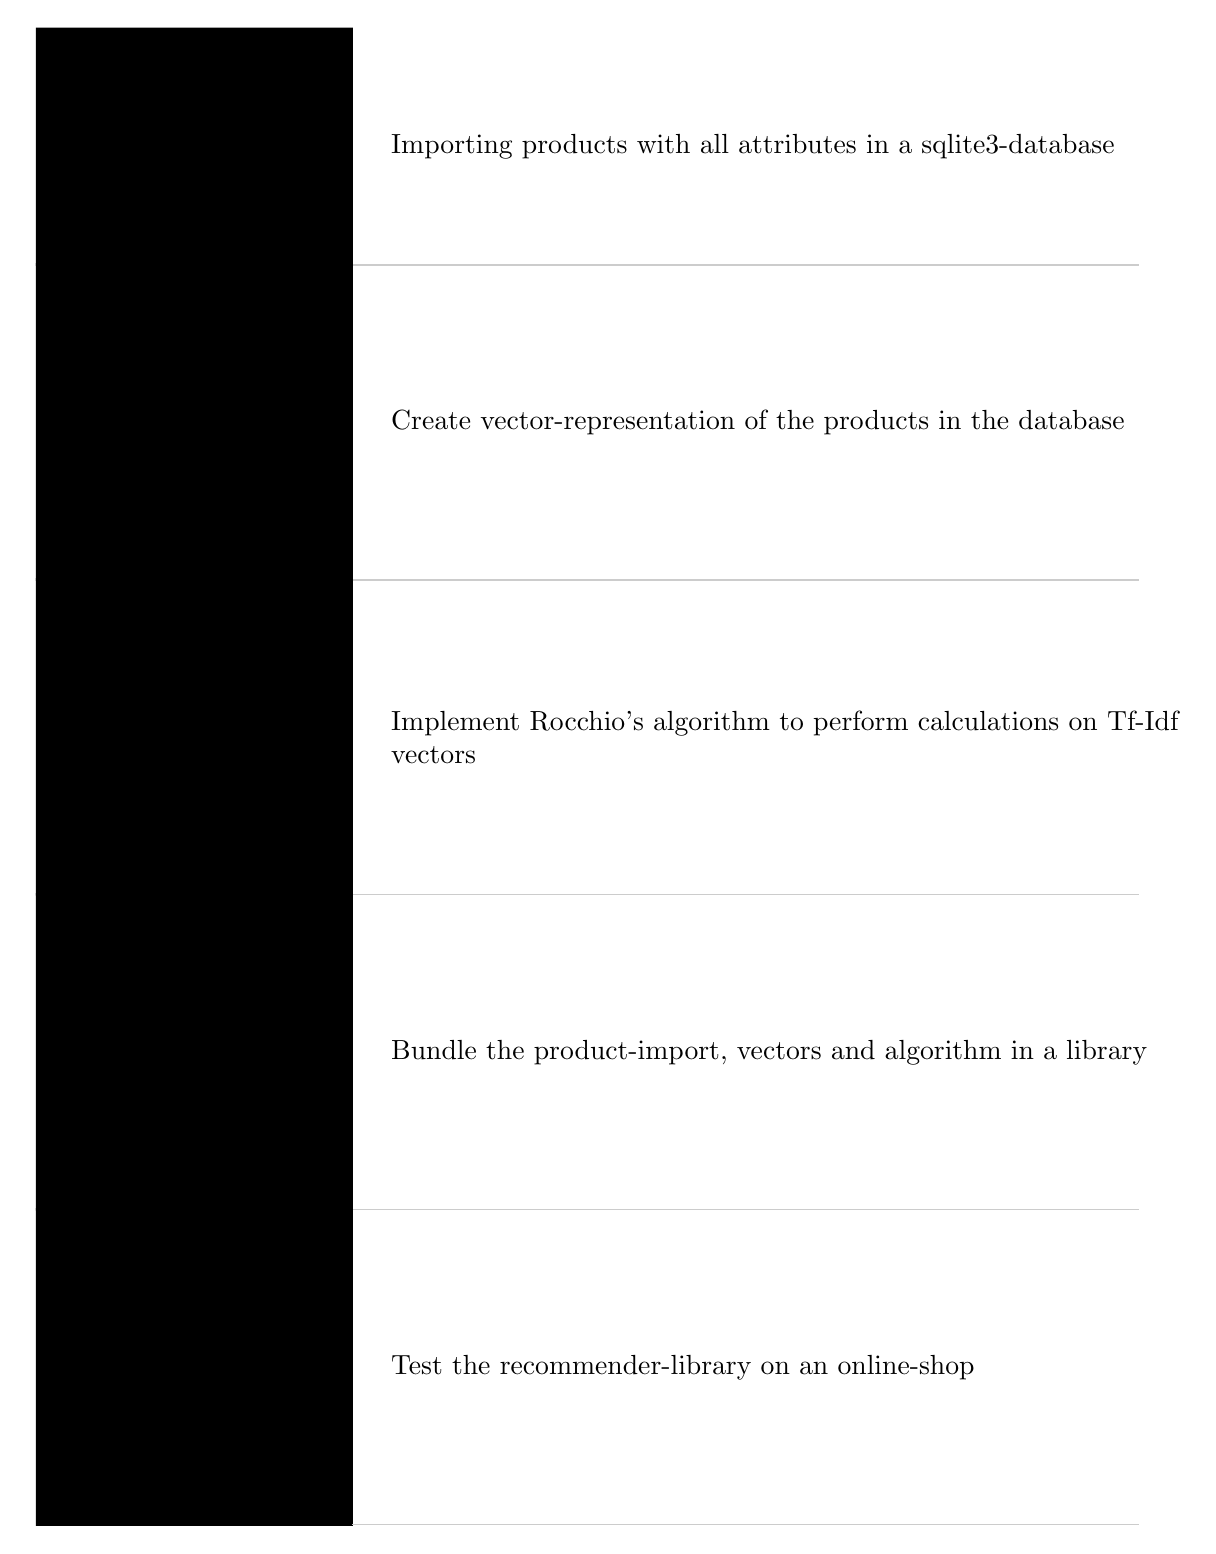
\begin{tikzpicture}
        %\def\dustTempLineWidth{12cm}
        \def\dustTempLineWidth{10cm}
        \def\dustTempNodeWidth{4cm}
        %\def\dustTempNodeHeight{4cm}
        \def\dustTempNodeHeight{3cm}
        \def\dustTempArrowHeight{1cm}
        \def\dustTempYShift{0cm}
        \def\dustTempLineColour{Black!20}

        \def\dustTempYShift{0 * -1 * (\dustTempNodeHeight + \dustTempArrowHeight)}
        \draw[thick,fill=\dustRowFirst]
            (0,0)--(\dustTempNodeWidth /2,-1* \dustTempArrowHeight)--(\dustTempNodeWidth,0)--(\dustTempNodeWidth,\dustTempNodeHeight)--(0,\dustTempNodeHeight)--cycle;
        \node[text width=\dustTempNodeWidth,text centered,yshift=\dustTempYShift] at (\dustTempNodeWidth /2,\dustTempNodeHeight /2)
        {
            \textbf{Import of products}
        };
        \node[text width=\dustTempLineWidth,align=left,yshift=\dustTempYShift] at ({\dustTempNodeWidth + \dustTempLineWidth /2 + 0.5cm},\dustTempNodeHeight/2)
        {
            Importing products with all attributes in a sqlite3-database
        };
        \draw[thin,\dustTempLineColour,yshift=\dustTempYShift] (\dustTempNodeWidth,0)--(\dustTempNodeWidth + \dustTempLineWidth,0);

        \def\dustTempYShift{1 * -1 * (\dustTempNodeHeight + \dustTempArrowHeight)}
        \draw[thick,fill=\dustRowSecond,yshift=\dustTempYShift]
            (0,0)--(\dustTempNodeWidth /2,-1 * \dustTempArrowHeight)--(\dustTempNodeWidth,0)--(\dustTempNodeWidth,\dustTempNodeHeight+\dustTempArrowHeight)--(\dustTempNodeWidth /2,\dustTempNodeHeight)--(0,\dustTempNodeHeight + \dustTempArrowHeight)--cycle;
        \node[text width=\dustTempNodeWidth,text centered,yshift=\dustTempYShift] at (\dustTempNodeWidth /2,\dustTempNodeHeight /2)
        {
            \textbf{Creation of vectors}
        };
        \node[text width=\dustTempLineWidth,align=left,yshift=\dustTempYShift] at ({\dustTempNodeWidth + \dustTempLineWidth /2 + 0.5cm},\dustTempNodeHeight /2 + \dustTempArrowHeight /2)
        {
            Create vector-representation of the products in the database
        };
        \draw[thin,\dustTempLineColour,yshift=\dustTempYShift] (\dustTempNodeWidth,0)--(\dustTempNodeWidth + \dustTempLineWidth,0);

        \def\dustTempYShift{2 * -1 * (\dustTempNodeHeight + \dustTempArrowHeight)}
        \draw[thick,fill=\dustRowFirst,yshift=\dustTempYShift]
        (0,0)--(\dustTempNodeWidth /2,-1 * \dustTempArrowHeight)--(\dustTempNodeWidth,0)--(\dustTempNodeWidth,\dustTempNodeHeight+\dustTempArrowHeight)--(\dustTempNodeWidth /2,\dustTempNodeHeight)--(0,\dustTempNodeHeight + \dustTempArrowHeight)--cycle;
        \node[text width=\dustTempNodeWidth,text centered,yshift=\dustTempYShift] at (\dustTempNodeWidth /2,\dustTempNodeHeight /2)
        {
            \textbf{Implementing recommender algorithm}
        };
        \node[text width=\dustTempLineWidth,align=left,yshift=\dustTempYShift] at ({\dustTempNodeWidth + \dustTempLineWidth /2 + 0.5cm},\dustTempNodeHeight /2 + \dustTempArrowHeight /2)
        {
            Implement Rocchio's algorithm to perform calculations on Tf-Idf vectors
        };
        \draw[thin,\dustTempLineColour,yshift=\dustTempYShift] (\dustTempNodeWidth,0)--(\dustTempNodeWidth + \dustTempLineWidth,0);

        \def\dustTempYShift{3 * -1 * (\dustTempNodeHeight + \dustTempArrowHeight)}
        \draw[thick,fill=\dustRowSecond,yshift=\dustTempYShift]
        (0,0)--(\dustTempNodeWidth /2,-1 * \dustTempArrowHeight)--(\dustTempNodeWidth,0)--(\dustTempNodeWidth,\dustTempNodeHeight+\dustTempArrowHeight)--(\dustTempNodeWidth /2,\dustTempNodeHeight)--(0,\dustTempNodeHeight + \dustTempArrowHeight)--cycle;
        \node[text width=\dustTempNodeWidth,text centered,yshift=\dustTempYShift] at (\dustTempNodeWidth /2,\dustTempNodeHeight /2)
        {
            \textbf{Create library}
        };
        \node[text width=\dustTempLineWidth,align=left,yshift=\dustTempYShift] at ({\dustTempNodeWidth + \dustTempLineWidth /2 + 0.5cm},\dustTempNodeHeight /2 + \dustTempArrowHeight /2)
        {
            Bundle the product-import, vectors and algorithm in a library
        };
        \draw[thin,\dustTempLineColour,yshift=\dustTempYShift] (\dustTempNodeWidth,0)--(\dustTempNodeWidth + \dustTempLineWidth,0);

        \def\dustTempYShift{4 * -1 * (\dustTempNodeHeight + \dustTempArrowHeight)}
        \draw[thick,fill=\dustRowFirst,yshift=\dustTempYShift]
            (0,0)--(\dustTempNodeWidth,0)--(\dustTempNodeWidth,\dustTempNodeHeight + \dustTempArrowHeight)--(\dustTempNodeWidth /2,\dustTempNodeHeight)--(0,\dustTempNodeHeight + \dustTempArrowHeight)--cycle;
        \node[text width=\dustTempNodeWidth,text centered,yshift=\dustTempYShift]at (\dustTempNodeWidth /2,\dustTempNodeHeight /2)
        {
            \textbf{Set up online-shop}
        };
        \node[text width=\dustTempLineWidth,align=left,yshift=\dustTempYShift] at ({\dustTempNodeWidth + \dustTempLineWidth /2 + 0.5cm},\dustTempNodeHeight /2 + \dustTempArrowHeight /2)
        {
            Test the recommender-library on an online-shop
        };
        \draw[thin,\dustTempLineColour,yshift=\dustTempYShift] (\dustTempNodeWidth,0)--(\dustTempNodeWidth + \dustTempLineWidth,0);

    \end{tikzpicture}

    \caption{Software milestones for building a recommender system}
    \label{fig:softwaremilestones}
\end{figure}

